\section{Cross-Protocol Comparison}
\label{sec:comparison}

This section presents the master comparison artifacts:
Table~\ref{tab:rubric-matrix}, Figure~\ref{fig:heatmap},
and Figure~\ref{fig:radar}. It then reads three structural
findings out of them. Section~\ref{sec:comparison:matrix}
walks the matrix axis-by-axis. Section~\ref{sec:comparison:clusters}
identifies the three protocol clusters the rubric makes
visible: registry-anchored, DID-anchored, and
commerce-settlement. Section~\ref{sec:comparison:stack}
returns to the layered-composition argument of
\S\ref{sec:taxonomy:complementary} and identifies where the
thirteen protocols overlap (and compete) versus where they
stack (and compose).

\subsection{The rubric-based comparison matrix}
\label{sec:comparison:matrix}

Table~\ref{tab:rubric-matrix} renders the eight
peer-messaging protocols of the survey against the ten
rubric axes. The five commerce-settlement protocols (AP2,
Visa TAP, Mastercard Agent Pay, ERC-8004, UCP) are treated
separately in \S\ref{sec:emerging:commerce} because the
peer-messaging rubric does not apply to them; their
structural comparison appears in
Table~\ref{tab:commerce-stack}. All eight remaining
protocols carry full scores. Six were scored at the
2026-Q1 cutoff (Google A2A, MCP, ANP, Coral, LOKA, ACNBP).
Two, IBM ACP and AGNTCY, were scored in a later pass and
are dated separately in
\texttt{protocol-scores.yaml}, because each required
reading a source the first pass had not: ACP's
OpenAPI~\cite{spec_openapi} document, and the four separate
AGNTCY specifications.
Per-axis evidence for every cell, including the
specification section each score rests on, is in the
evidence field of \texttt{data/protocol-scores.yaml} in the
companion repository.

% Generated by scripts/gen_table1.py: do NOT hand-edit.
% Source: data/protocol-scores.yaml.

\begin{table*}[t]
  \centering
  \caption{Master rubric matrix. Ordinal axes (A1 to A3, A5 to A7, A9) use anchored descriptors 0 to 3. Threat-surface (A8) is a count N/12. Transport (A4) is a tuple (serialization summarized). Governance (A10) is the composite triple \textit{steward / license / observability}. Scores are not summed; see \S\ref{sec:rubric}.}
  \label{tab:rubric-matrix}
  \footnotesize
  \textit{Panel (a): axes A1 to A5}\par\smallskip
  \resizebox{\textwidth}{!}{%
  \begin{tabular}{p{4.2cm}cccp{5.0cm}c}
    \toprule
    Protocol & A1 & A2 & A3 & A4 & A5 \\
    \midrule
    \textbf{Google A2A} & \score{1} & \score{1} & \score{1} & \scriptsize HTTPS/JSON-RPC 2.0, optional g & \score{3} \\
    \textbf{Model Context Protocol (MCP)} & \score{1} & \score{1} & \score{1} & \scriptsize stdio, HTTP+SSE, streamable-HT & \score{1} \\
    \textbf{Agent Network Protocol (ANP)} & \score{3} & \score{3} & \score{2} & \scriptsize HTTPS & \score{1} \\
    \textbf{IBM ACP / BeeAI} & \score{1} & \score{1} & \score{1} & \scriptsize HTTP/REST & \score{3} \\
    \textbf{AGNTCY / SLIM (Cisco-led)} & \score{3} & \score{2} & \score{1} & \scriptsize gRPC over HTTP/2, HTTP/3 & \score{1} \\
    \textbf{Coral Protocol} & \score{2} & \score{3} & \score{2} & \scriptsize HTTP, WebSocket, SSE & \score{2} \\
    \textbf{LOKA Protocol} & \score{3} & \score{3} & \score{2} & \scriptsize unspecified & \score{2} \\
    \textbf{Agent Capability Negotiation and Binding Protocol} & \score{2} & \score{2} & \score{2} & \scriptsize unspecified at link level & \score{3} \\
    \bottomrule
  \end{tabular}%
  }
  \par\medskip
  \textit{Panel (b): axes A6 to A10}\par\smallskip
  \resizebox{\textwidth}{!}{%
  \begin{tabular}{p{4.2cm}ccccp{6.0cm}}
    \toprule
    Protocol & A6 & A7 & A8 & A9 & A10 \\
    \midrule
    \textbf{Google A2A} & \score{3} & \score{3} & \score{1/12} & \score{1} & \scriptsize Linux Foundation / Apache 2.0 / obs=2 \\
    \textbf{Model Context Protocol (MCP)} & \score{2} & \score{2} & \score{1/12} & \score{1} & \scriptsize Linux Foundation AAIF / MIT-equivalent / obs=1 \\
    \textbf{Agent Network Protocol (ANP)} & \score{1} & \score{1} & \score{5/12} & \score{2} & \scriptsize community / W3C-aligned / Apache 2.0 / obs=1 \\
    \textbf{IBM ACP / BeeAI} & \score{2} & \score{2} & \score{1/12} & \score{1} & \scriptsize LF AI \& Data (archived) / Apache 2.0 / obs=2 \\
    \textbf{AGNTCY / SLIM (Cisco-led)} & \score{3} & \score{0} & \score{6/12} & \score{2} & \scriptsize Linux Foundation / Apache 2.0 / obs=3 \\
    \textbf{Coral Protocol} & \score{2} & \score{0} & \score{3/12} & \score{1} & \scriptsize Coral Protocol team / CC-BY-4.0 (paper) / obs=2 \\
    \textbf{LOKA Protocol} & \score{3} & \score{1} & \score{6/12} & \score{3} & \scriptsize academic authors (CMU Tepper / BIT Sindri); no formal SDO / CC-BY-NC-SA 4.0 / obs=3 \\
    \textbf{Agent Capability Negotiation and Binding Protocol} & \score{2} & \score{1} & \score{10/12} & \score{2} & \scriptsize individual authors (DistributedApps.ai, Cisco, OWASP/AWS, Intuit); no formal SDO / CC-BY 4.0 / obs=3 \\
    \bottomrule
  \end{tabular}%
  }
\end{table*}


Three observations stand out from the matrix.

\paragraph{No protocol scores uniformly high.}
The strongest single profile is ACNBP, which combines an
Axis 5 score of 3 (the ten-step state machine) with the
highest Axis 8 threat count of the surveyed set
(10/12). It nevertheless scores 2 on Axis 1 (federated
directory rather than DID-resolver) and 1 on Axis 7
(typed capability parameters without inline
multimodal). LOKA scores 3 on every ordinal axis except 5
and 7 but pays for that profile with Axis 4's
\texttt{unspecified} transport row: the score is
aspirational. A2A pairs three 3s (axes 5, 6, 7) with three
1s (axes 1, 2, 3); ANP inverts that profile, pairing
identity-layer 3s with task-and-content-layer 1s. The
matrix renders an observation that no prior survey could
make precise: \emph{the contemporary protocols specialize
into mutually-exclusive strengths, and no surveyed protocol
combines a deployed task model with a decentralized
identity model.}

% Commerce-settlement co-stack: hand-authored from \S6.3 source material.
% Not generated from YAML; the peer-messaging rubric does not apply to
% these protocols. See manuscript/sections/06-emerging-protocols.tex
% (\S\ref{sec:emerging:commerce}) for the structural analysis.

\begin{table}[h!]
  \centering
  \caption{Commerce-settlement co-stack at the 2026-Q1 cutoff. The first four
  protocols share the intent-mandate-receipt envelope pattern
  (\S\ref{sec:emerging:commerce}) but bind it to different settlement
  substrates and mandate encodings. UCP is the exception and is listed last:
  it binds no substrate of its own and consumes AP2's mandate through an
  optional extension, which is why its row reads \emph{none of its own}. The
  peer-messaging rubric (\S\ref{sec:rubric}) does not apply to any of the
  five; this table captures the structural axes on which they actually
  differentiate.}
  \label{tab:commerce-stack}
  \footnotesize
  \begin{tabular}{lllll}
    \toprule
    Protocol & Steward & Settlement Substrate & Mandate Encoding & Anchor \\
    \midrule
    AP2                  & PayPal + Google           & PayPal payment rails (ref.\ impl.) & Typed off-chain envelope          & off-chain \\
    Visa TAP             & Visa                      & Visa card network                  & EMVCo-aligned authorization       & off-chain \\
    Mastercard Agent Pay & Mastercard                & Mastercard card network            & Mirrors Visa TAP pattern          & off-chain \\
    ERC-8004             & Ethereum (EIP authors)    & Ethereum / EVM blockchain          & Smart contract + tx receipt       & on-chain  \\
    UCP                  & Google + Shopify councils & none of its own (delegated)        & AP2 mandate, optional extension   & off-chain \\
    \bottomrule
  \end{tabular}
\end{table}


\paragraph{The Axis 3 gap is the central open problem.}
No protocol in the scored set reaches Axis~3 level~3. The
column has no upper cell occupied. A2A, MCP, ACP, and
AGNTCY sit at 1 (scope tokens or short-lived bearer
tokens, with no standardised delegation credential). ANP,
Coral, LOKA, and ACNBP sit at 2 (VC-scoped capabilities,
smart-contract policies, or a two-party binding ceremony,
in each case without a standardized chain-of-custody
format). The two protocols added to the scored set do not
disturb the result: ACP specifies no authorization
primitive at all despite documenting hierarchical agent
composition, and AGNTCY pairs MLS group membership with
short-lived OAuth bearer tokens.

The gap is therefore universal rather than
near-universal, and that is the stronger claim. It holds
even for ACNBP, which carries the highest threat-coverage
count in the survey and an explicit MAESTRO threat
analysis. Rigour on one hop does not produce a chain. A
specification can bind a caller to a callee with mutual
signatures, an attestation, and an immutable audit trail,
and still leave a downstream agent unable to verify where
the authority came from. The literature on this
gap~\cite{authz_propagation, agentic_jwt, did_vc_agents}
is converging on the agentic-JWT pattern or an analogue,
and the commerce-settlement layer already reaches level 3
through its mandate envelope
(\S\ref{sec:emerging:commerce}), but no peer-messaging
protocol has adopted either into the specification.
Section~\ref{sec:openproblems} returns to
this gap as the single highest-priority item on the
open-problems agenda.

\begin{figure*}[t]
  \centering
  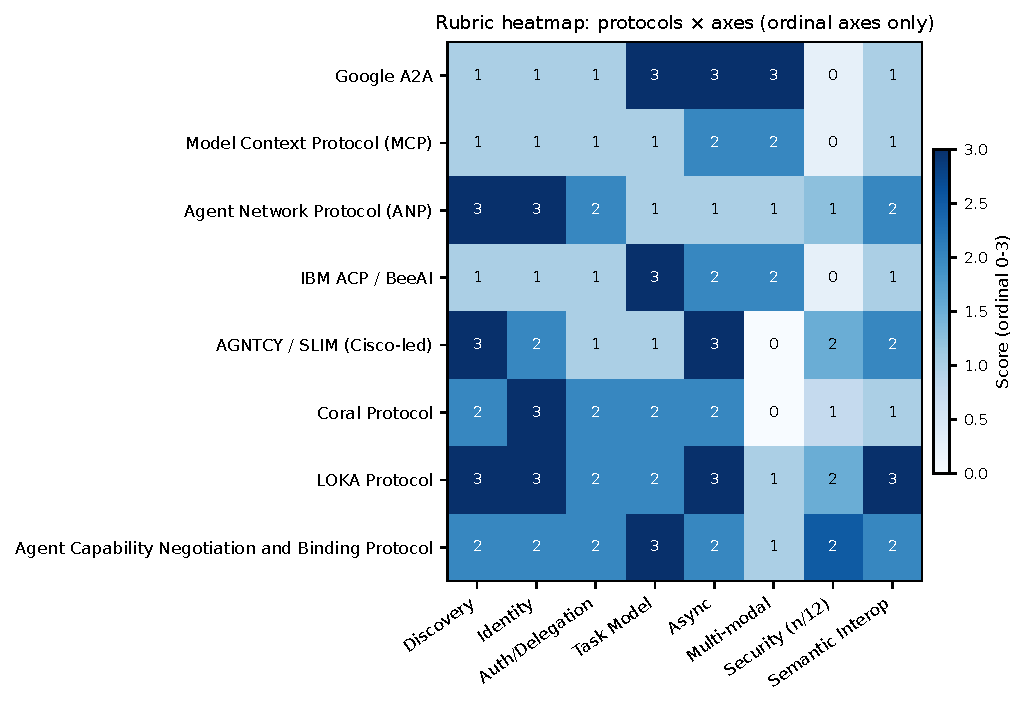
\includegraphics[width=0.85\textwidth]{figures/fig5-heatmap.pdf}
  \caption{Rubric heatmap across protocols and axes. Colour
  encodes the ordinal score for axes 1 to 3, 5 to 7, and 9;
  axes 4, 8, and 10 are summarized as described in
  \S\ref{sec:rubric}. Empty rows are pending per-protocol
  evidence notes for the two placeholder protocols (IBM ACP,
  AGNTCY/SLIM); the five commerce-settlement protocols are
  scored separately in Table~\ref{tab:commerce-stack}. The
  matrix is regenerated mechanically
  from \texttt{data/protocol-scores.yaml} by
  \texttt{scripts/gen\_heatmap.py}.}
  \label{fig:heatmap}
\end{figure*}

\begin{figure*}[!ht]
  \centering
  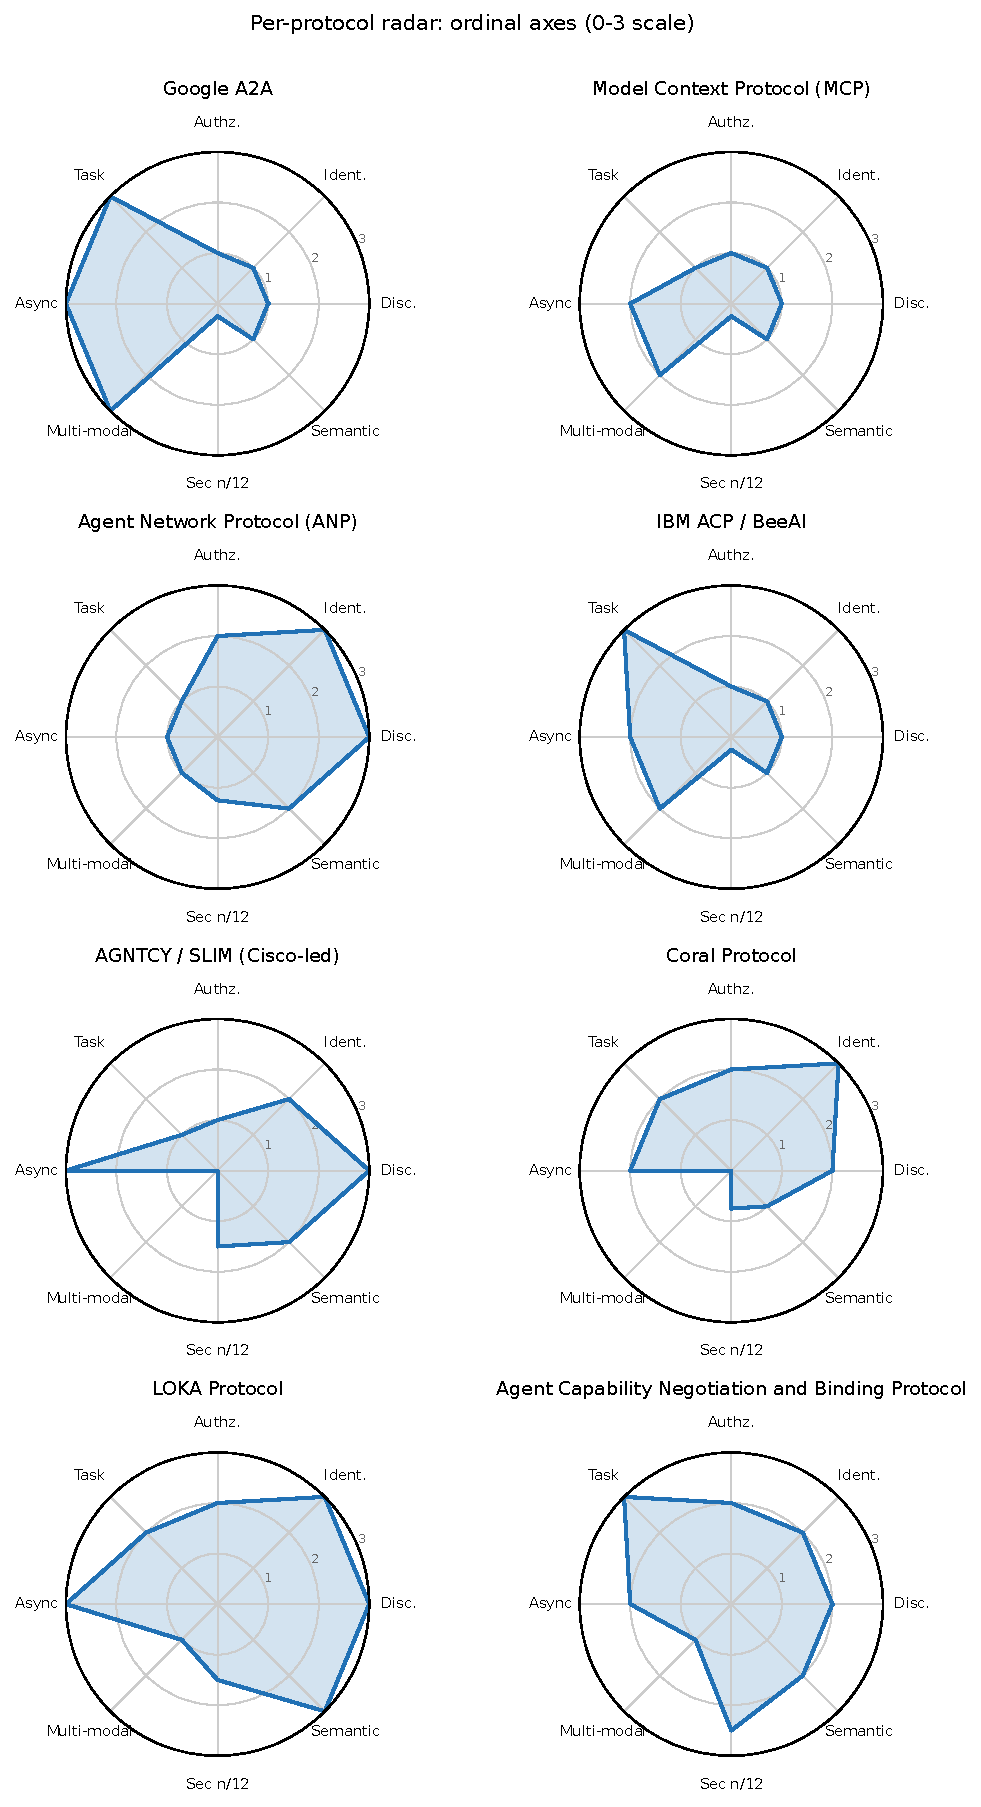
\includegraphics[width=0.75\textwidth]{figures/fig6-radar.pdf}
  \caption{Per-protocol radar charts on the seven ordinal
  axes (1 to 3, 5 to 7, 9) plus a normalized Axis 8 threat
  count. Each polygon describes a protocol's profile across
  the rubric; the heatmap (Figure~\ref{fig:heatmap})
  presents the same data as a colour matrix for
  cross-protocol comparison. Regenerated by
  \texttt{scripts/gen\_radar.py}.}
  \label{fig:radar}
\end{figure*}

\paragraph{The Axis 9 gap is structural.}
No surveyed protocol scores 3 on semantic interoperability.
LOKA's score of 3 is explicitly aspirational; the
Polyglot Intent Engine is a proposed mechanism rather than
a shipped one. Five protocols (A2A, MCP, ACP, Coral, and
the Axis-9 aspect of AGNTCY) cluster at 1 (free-text
descriptions over typed schemas). ANP at level 2
(JSON-LD with ADP) is the only protocol that
\emph{ships} an ontology-base mechanism. The gap is
discussed in detail in \S\ref{sec:semantic}; the rubric
makes precise that the LLM-era flexibility we celebrated
in \S\ref{sec:background:llm-disruption} has come at a
documented cost on this axis.

\subsection{How each score was assigned: per-axis derivation}
\label{sec:comparison:derivation}

This subsection walks every axis in Table~\ref{tab:rubric-matrix}
and explains, cell-by-cell, what specification evidence
anchored each scored protocol at the level shown. The
methodology is the four-step procedure of
\S\ref{sec:rubric:method}: identify the spec section
relevant to the axis, map its behaviour to the anchored
descriptors of \S\ref{sec:rubric:axes}, record the
resulting score, and write the evidence summary. Each
paragraph below corresponds to one column of the
comparison matrix. The companion repository's
\texttt{data/protocol-scores.yaml} carries the
machine-readable form of every evidence sentence quoted
here, with the spec citation key attached.

\paragraph{Axis 1 (Discovery and Registry Model).}
Recall the anchored descriptors of \S\ref{sec:rubric:axis1}:
0 = out-of-band only; 1 = well-known endpoint; 2 =
federated directory with structured descriptors; 3 =
decentralized verifiable resolution. \textbf{A2A scores 1}
because its discovery primitive is the well-known endpoint
\texttt{/.well-known/agent-card.json}~\cite{spec_a2a};
trust is delegated to the hosting authority and no
verifiable cryptographic resolution is provided.
\textbf{MCP also scores 1}: the spec defines
server-config-mediated discovery with an emerging registry
that is, at the cutoff, mostly out-of-band~\cite{spec_mcp};
the level-1 anchor (configuration mediated) fits more
naturally than level 0. \textbf{ANP scores 3}: the white
paper specifies a DID resolver paired with the Agent
Description Protocol, returning cryptographically
verifiable descriptors independent of any single
authority~\cite{spec_anp}. \textbf{Coral scores 2}: the
\texttt{list\_agents} MCP tool resolves names from a
server-mediated Coral Server; the resolution is
blockchain-anchored but server-mediated rather than
DID-based~\cite{spec_coral}, fitting the federated-directory
anchor. \textbf{LOKA scores 3}: its Semantic Discovery
Fabric (\S3.2 of the LOKA white paper) plus the proposed
\texttt{did:loka:} resolver in \S4.1 match the
decentralized-verifiable-resolution descriptor~\cite{spec_loka};
the score is aspirational, as flagged in
\S\ref{sec:rubric:limits}, but the specification text
supports the level. \textbf{ACNBP scores 2}: Definition~4
of the spec defines the Agent Name Service as a
DNS-like federated directory maintaining Agent Network
Resource Identifiers~\cite{spec_acnbp}; federated but not
DID-based, hence level 2.

\paragraph{Axis 2 (Identity and Authentication).}
Anchors of \S\ref{sec:rubric:axis2}: 0 = process trust or
unspecified; 1 = bearer tokens (OAuth-style); 2 = bearer
tokens hardened with mTLS or signed envelopes; 3 = DIDs
with verifiable credentials. \textbf{A2A scores 1}: OAuth
2.x is documented in the AgentCard schema; mTLS and JWT
are supported but not mandated, and the spec does not
require message-level signing~\cite{spec_a2a, a2a_weaknesses}.
\textbf{MCP scores 1}: OAuth 2.1 is the HTTP-transport
identity mechanism; the stdio transport relies on
parent-process trust, which the rubric records as a
level-1 hybrid in the evidence field~\cite{spec_mcp}.
\textbf{ANP scores 3}: identity is established by DIDs
plus W3C Verifiable Credentials, the rubric's level-3
anchor~\cite{spec_anp}. \textbf{Coral scores 3}: each
agent holds a DID with cryptographic credentials, and
Solana wallets serve as the authenticator (\S7 of the
Coral paper)~\cite{spec_coral}, matching the
DID-with-VC anchor. \textbf{LOKA scores 3}: \S4.1
specifies DID documents with Ed25519 keys plus VCs with
issuer/subject/verifier roles and a Dilithium post-quantum
upgrade path~\cite{spec_loka}. \textbf{ACNBP scores 2}:
identity rests on X.509 certificates with OCSP revocation
and ECC-signed envelope structures (\S\S III.A, IV.A,
VII.B)~\cite{spec_acnbp}; DIDs are not native, but the
combination of signed envelopes with PKI matches the
level-2 anchor, not level 3.

\paragraph{Axis 3 (Authorization and Delegation Model).}
Anchors of \S\ref{sec:rubric:axis3}: 0 = unspecified; 1 =
scope tokens, or no standardised delegation credential;
2 = VC-scoped
capabilities or structured delegation tokens; 3 =
cryptographically-bound capability chains. \textbf{A2A
scores 1}: the spec advertises authentication schemes in
the AgentCard and defines an in-task authorization flow
(\S7.6) with an auth-required task state, but standardises
no delegation credential. \S7.5 makes authorization logic
implementation-specific~\cite{spec_a2a}. The in-task flow
re-acquires a credential at the boundary rather than
carrying a verifiable chain, so the receiver still holds a
bearer credential with no chain of custody behind it. That
is the level-1 anchor. Deployments close the gap with
token forwarding, which the security literature observes
in production~\cite{authz_propagation}; the pattern is
attributable to deployments, not to the specification. \textbf{MCP
scores 1}: OAuth scopes only; no agent-delegation
primitive in the cutoff spec~\cite{spec_mcp}.
\textbf{ANP scores 2}: VC-scoped capabilities are
supported and cryptographic chains are possible in
principle, but the chain-of-custody pattern is not fully
standardized~\cite{spec_anp}. \textbf{Coral scores 2}:
\S7 defines Team Contracts as signed multi-agent
agreements (optionally on-chain); this is a partial
delegation chain, not yet at the level of RFC
8693~\cite{rfc8693} or better~\cite{spec_coral}.
\textbf{LOKA scores 2}: VCs act as scoped capability
attestations (\S4.1) and smart-contract lifecycle
policies (\S3.1) carry the policy layer; no RFC 8693
mapping~\cite{spec_loka}. \textbf{ACNBP scores 2}:
Definition~10 defines Capability Binding as a
cryptographically-bound, mutually-signed commitment
backed by a capability attestation (Def.~14) with
immutable audit trails~\cite{spec_acnbp}. This is the
most rigorous single-hop authorization primitive in the
surveyed set, and it is single-hop. Definition~10 binds a
requester agent to a provider agent, two named parties.
The specification does not extend the binding to a third
party, and its text contains no treatment of delegation,
authorization propagation, or acting on behalf of another
principal. A lead author confirmed in correspondence that
ACNBP is a two-party negotiation-and-binding protocol and
that multi-agent delegation is outside its scope. So the
level-3 clause requiring an intermediate agent's
authorization to be independently verifiable is
unsatisfied, and the cell records level 2. This is the
last ordinal-3 the Axis 3 column had, and with it the
column tops out at 2
(\S\ref{sec:emerging:acnbp} gives the full derivation).

\paragraph{Axis 4 (Transport and Wire Format).}
Recall this axis is a tuple rather than an ordinal score
(\S\ref{sec:rubric:axis4}). The cells record what the
specification declares, not what implementations support.
A2A: HTTPS/JSON-RPC 2.0 with optional gRPC and REST,
JSON serialization, SSE streaming, push
notifications~\cite{spec_a2a}. MCP: stdio, HTTP+SSE, and
streamable-HTTP bindings; JSON-RPC 2.0 serialization;
SSE or chunked HTTP streaming; notifications plus
emerging MCP Tasks~\cite{spec_mcp}. ANP: HTTPS only;
JSON-LD over JSON; no native streaming; polling for
async~\cite{spec_anp}. Coral: HTTP / WebSocket / SSE;
JSON-via-MCP; SSE streaming; push via
\texttt{wait\_for\_mentions}~\cite{spec_coral}. LOKA:
\texttt{unspecified} on every sub-field. The paper
declares intent-centric peer-to-peer messaging
without committing to a transport binding~\cite{spec_loka}.
ACNBP: unspecified at the link layer (the spec is
transport-agnostic), JSON serialization
(RFC 7159~\cite{rfc7159}), no
in-protocol streaming, and a 10-step asynchronous
negotiation with encrypted session and forward
secrecy~\cite{spec_acnbp}. The tuple values are
transcribed verbatim from the spec sections cited in
the YAML evidence field; transcription is the only
rubric methodology for this axis. The RFC 7159 reference
is the specification's own, and it is stale: RFC 8259
obsoleted that revision in 2017.

\paragraph{Axis 5 (Task and Conversation Model).}
Anchors of \S\ref{sec:rubric:axis5}: 0 = stateless
request/response; 1 = session-scoped but no task object;
2 = persistent multi-participant interaction; 3 = full
task object with lifecycle, artifacts, and sub-task
delegation. \textbf{A2A scores 3}: the \texttt{Task}
object carries a lifecycle (submitted, working,
input-required, completed, failed, canceled), Parts and
Artifacts content aggregation, and explicit sub-task
delegation~\cite{spec_a2a}. \textbf{MCP scores 1}:
request/response with session-scoped state; the emerging
MCP Tasks extension begins to push toward level 2 but
is post-cutoff~\cite{spec_mcp}. \textbf{ANP scores 1}:
multi-turn interaction is supported, but a task is not a
protocol-level concept~\cite{spec_anp}. ANP's first-class
concepts are Information and Interface, and a task is
treated as one form of an Interface, on the argument that
the task abstraction is not general enough to carry every
interaction (\S\ref{sec:industry:anp}). The level records
the absence of the object, not an unfinished lifecycle. \textbf{Coral
scores 2}: stateful persistent multi-participant threads
are first-class; sub-task delegation is deferred to a
future Task Management service (\S7)~\cite{spec_coral}.
\textbf{LOKA scores 2}: the ALMS lifecycle (Genesis,
Growth, Crisis, Sunset) in \S3.1 covers agent lifecycle;
sub-task delegation is discussed in \S4.4.3 but is not a
first-class task primitive~\cite{spec_loka}.
\textbf{ACNBP scores 3}: the ten-step state machine of
the spec, with Protocol State (Def.~15) as a first-class
object, binding commitments that produce artifacts, and
multi-agent orchestration with capability composition
(\S IV.A), matches the level-3 anchor~\cite{spec_acnbp}.

\paragraph{Axis 6 (Async and Long-Running Operations).}
Anchors of \S\ref{sec:rubric:axis6}: 0 = no async; 1 =
polling-based; 2 = server-initiated notifications; 3 =
durable resumable tasks. \textbf{A2A scores 3}: push
notifications combine with polling and durable resumable
tasks; on reconnect the client receives a complete or
partial result and any backfilled events~\cite{spec_a2a}.
\textbf{MCP scores 2}: notifications plus emerging MCP
Tasks; durability across connection loss is not yet a
cutoff-specification feature~\cite{spec_mcp}. \textbf{ANP
scores 1}: polling primarily; the white paper does not
specify a push-notification standard~\cite{spec_anp}.
Asynchrony is left to the individual Interface to define
rather than raised to a protocol-level primitive, so the
level reflects a scoping decision
(\S\ref{sec:industry:anp}).
\textbf{Coral scores 2}: \texttt{wait\_for\_mentions} is
an explicit push primitive (\S6.1.2); durable-resumable
semantics are not specified~\cite{spec_coral}.
\textbf{LOKA scores 3}: \S3.1 specifies Crisis-phase
continuous checkpointing, redundancy overlays, and
recovery via verifiable snapshots, matching the
durable-resumable anchor (aspirationally)~\cite{spec_loka}.
\textbf{ACNBP scores 2}: \S IV.A specifies
subscription-based capability update notifications;
durable-resumable bound execution is not
specified~\cite{spec_acnbp}.

\paragraph{Axis 7 (Multi-Modal Content Handling).}
Anchors of \S\ref{sec:rubric:axis7}: 0 = plain text;
1 = text plus referenced attachments; 2 = typed content
blocks; 3 = typed parts with inline-or-reference duality.
\textbf{A2A scores 3}: TextPart, FilePart, and DataPart
with inline and URL-reference modes are the canonical
level-3 vocabulary~\cite{spec_a2a}. \textbf{MCP scores
2}: typed content blocks (text, image, resource) plus
structured JSON-Schema tool input fit the level-2
anchor~\cite{spec_mcp}; level 3 would require explicit
content negotiation. \textbf{ANP scores 1}: text plus
file references; no typed parts model~\cite{spec_anp}.
\textbf{Coral scores 0}: natural-language message content
with mention metadata only; no typed parts, file
references, or content negotiation
schema~\cite{spec_coral}. This is the lowest score on
Axis 7 in the surveyed set and the largest single weak
spot in Coral's profile. \textbf{LOKA scores 1}: the
DID document defines a CredentialRepositoryService with
a service endpoint URL (\S4.1); typed inline multimodal
parts are not specified~\cite{spec_loka}. \textbf{ACNBP
scores 1}: capabilities define typed input/output
parameters (Def.~2) but the spec does not specify
inline multimodal parts or streaming media~\cite{spec_acnbp}.

\paragraph{Axis 8 (Security Threat Surface).}
This axis is a count over the fixed twelve-item threat
catalogue of \S\ref{sec:rubric:axis8}. Counts are the
number of threats that the specification \emph{explicitly}
addresses at the spec level, not at the deployment level.
A mitigation that the specification recommends without
requiring scores \emph{partial} and does not enter the
count, which is why several counts here are lower than a
reading of the same protocol's security section suggests.
\textbf{A2A: 3 partial, 1 of 12 addressed}: transport
encryption is the sole spec-level mitigation. OAuth bearer
identity, push-notification replay verification, and
transport-layer DoS resistance are real but partial:
the AgentCard itself is unsigned. Injection, AgentCard
supply-chain attacks,
registry poisoning, and delegation token theft are
explicitly identified as out-of-spec in the
literature~\cite{a2asecbench, a2a_weaknesses, spec_a2a}.
\textbf{MCP: 2 partial, 1 of 12 addressed}: TLS on the HTTP
transport is the sole spec-level mitigation. OAuth 2.1
identity is partial because the stdio transport substitutes
process trust, and token expiry is the only replay defence.
Indirect injection and tool poisoning are
documented as unaddressed~\cite{zhan2024injecagent,
protocol_exploits, spec_mcp}. Two classes are not
applicable, since MCP is agent-to-tool rather than
peer-to-peer. \textbf{ANP: 5 of 12}:
identity, authentication, integrity, audit, and
non-repudiation are addressed through DIDs and VCs;
prompt injection, registry poisoning, and capability
escalation remain unaddressed~\cite{spec_anp}.
\textbf{Coral: 3 partial, 3 of 12 addressed}: DIDs and Solana wallet
authentication, on-chain immutable audit, and thread-scoped
privilege confusion are addressed. Team-contract capability
escalation and delegation token theft are partial, and so is
message integrity, because the on-chain signatures cover the
payment path and not the message path. Replay, supply-chain,
side-channel, DoS, prompt injection, and registry poisoning are
not addressed~\cite{spec_coral}. \textbf{LOKA: 4 partial, 6 of 12 addressed}:
DID-and-Dilithium authentication, timestamp-and-signed-intent
replay, blockchain audit, post-quantum MITM,
decentralized-SSI registry, and Contextual Ethics privilege
confusion are addressed. The DECP prompt-injection filter,
VC-and-contract capability scoping, delegation token
binding, and the Contextual Ethics privacy policies are
partial, so they do not enter the count. Supply-chain and
DoS are not addressed~\cite{spec_loka}. \textbf{ACNBP: 10 of
12}: the MAESTRO 7-layer analysis (\S VII.I) explicitly
addresses ZKP capability attestation, signature plus HMAC
integrity, rate-limit-plus-PoW DoS mitigation,
nonce-and-timestamp-and-sequence replay defence,
\texttt{protocolExtension} whitelist supply-chain
defence, X.509 plus OCSP impersonation defence, the
Capability Binding ceremony against delegation-token
theft, signed-ANRI plus BFT registry integrity,
foundation-model prompt-injection mitigation, and
cryptographically protected audit logs~\cite{spec_acnbp}.
Two classes score partial and do not enter the count:
side-channel privacy, offered through ring signatures,
and cross-agent privilege confusion, offered through
agent quarantine. The count is the
highest in the surveyed set; \S\ref{sec:security} returns
to the question of how to read a high count when the
underlying spec lacks production deployment.

\paragraph{Axis 9 (Semantic Interoperability).}
Anchors of \S\ref{sec:rubric:axis9}: 0 = free-text only;
1 = structured schemas with free-text descriptions; 2 =
ontology-base or semantic-discovery indexing; 3 = full
capability ontology with semantic matching. \textbf{A2A
scores 1}: typed Skill objects pair with free-text
descriptions and no ontology alignment~\cite{spec_a2a}.
\textbf{MCP scores 1}: JSON Schema for tool input with
free-text natural-language tool descriptions~\cite{spec_mcp}.
\textbf{ANP scores 2}: JSON-LD as the serialization
provides an ontology base, and ADP enables semantic
discovery~\cite{spec_anp}; the only ordinal-2 on Axis 9
in the surveyed set. This is the one cell in the matrix
that a post-cutoff revision would move
(\S\ref{sec:semantic:ontology}). \textbf{Coral scores 1}: Coraliser
adapters enforce uniform schemas (\S6.3) but the spec
does not specify a formal capability descriptor or
ontology~\cite{spec_coral}. \textbf{LOKA scores 3}: the
combination of capability ontologies, intent schemas,
ethical inheritance (\S3.1) and the Polyglot Intent
Engine targeting FIPA-ACL / A2A / Open Voice
(\S4.5.2)~\cite{spec_loka} matches the full-ontology
anchor aspirationally. The engine is not yet
implemented. \textbf{ACNBP scores 2}: Definition~2
provides a structured capability descriptor; \S IV.D
specifies a Semantic Consistency Check; ontology-based
classification (\S VIII.A) is recommended as a future
enhancement~\cite{spec_acnbp}.

\paragraph{Axis 10 (Governance, License, and Observability).}
The composite triple of \S\ref{sec:rubric:axis10} is
recorded by transcription rather than scoring for the
first two sub-fields; only the third (observability) is
ordinal. \textbf{A2A}: Linux Foundation steward, Apache
2.0 licensed, observability 2 (SSE event stream supports
tracing; no standardized audit
primitives)~\cite{spec_a2a, lf_aaif}. \textbf{MCP}:
Linux Foundation AAIF steward, MIT-equivalent licensed,
observability 1 (logging hooks emerging; no standardized
audit primitives)~\cite{spec_mcp, lf_aaif}.
\textbf{ANP}: community / W3C-aligned steward, Apache
2.0 licensed, observability 1 (built-in non-repudiation
logs; no standardized audit dashboard)~\cite{spec_anp,
w3c_agent_protocol_cg}. \textbf{Coral}: Coral Protocol
team steward, CC-BY-4.0 paper license, observability 2
(mandatory blockchain audit trail for payments and team
contracts in \S8; no separate trace or metric
spec)~\cite{spec_coral}. \textbf{LOKA}: academic-authors
steward (CMU Tepper / BIT Sindri) with no formal SDO,
CC-BY-NC-SA 4.0 licensed, observability 3 (\S5.1
specifies immutable audit trails, real-time ethical
auditing, and blockchain-ledger action and reasoning
records)~\cite{spec_loka}. \textbf{ACNBP}:
individual-authors steward (DistributedApps.ai, Cisco,
OWASP/AWS, Intuit) with no formal SDO, CC-BY 4.0
licensed, observability 3 (\S IV.H specifies
cryptographically protected audit logs, comprehensive
event logging, privacy-preserving logging, and
integration with external audit/compliance
systems)~\cite{spec_acnbp}. The composite is not
aggregated into a single number, by D3 of
\S\ref{sec:rubric:goals}; \S\ref{sec:governance} treats
governance as the most decisive of the three sub-fields
for protocol survival.

\paragraph{Contestable boundary calls.}
Four cells in Table~\ref{tab:rubric-matrix} sit at
contestable boundaries that a reader may dispute. \textbf{A2A on Axis 1.} A reader
who classes the AgentCard convention as a federation
rather than a hosted convention could plausibly raise
A2A to level 2; we score 1 because no central registry
is specified and the convention is implemented by each
host individually. \textbf{ANP on Axis 3.} A reader who
treats VC-scoped capabilities plus the implicit
cryptographic chain as a complete level-3 mechanism
could raise ANP to 3; we score 2 because the
chain-of-custody format is not standardized in the
white paper and no reference profile of the chain has
been published. \textbf{Coral on Axis 2.} A reader could
plausibly score Coral at 2 (signed envelopes via Solana
wallet signatures) rather than 3 (DIDs and VCs) by
arguing that the wallet signature is the operative
identity primitive and the DID is decorative; we score 3
because the spec text in \S7 establishes the DID as the
primary identifier and the wallet as the cryptographic
authenticator over it. \textbf{ACNBP on Axis 3.} A reader
who treats the capability-binding ceremony as satisfying
the level-3 anchor's parenthetical could score ACNBP at 3,
and an earlier version of this survey did. We score 2
because the anchor's operative clause is the one after the
parenthetical: an intermediate agent's authorization must
be independently verifiable, and Definition~10 binds only
two parties. A lead author confirmed the two-party reading
in correspondence, which agrees with the specification
text. This is the only cell in the matrix whose score
changed after correspondence with a protocol's authors,
and it is recorded as such in the YAML. Each of these
calls is flagged in the YAML evidence field so future
readers can re-litigate them against the
\texttt{spec\_version}/\texttt{retrieved} pair in effect.



\subsection{Clusters: registry-anchored, DID-anchored, commerce-settlement}
\label{sec:comparison:clusters}

The rubric matrix renders three protocol clusters that no
prior survey identified as architecturally distinct.

\paragraph{Cluster 1: Registry-anchored.}
A2A, MCP, ACP, AGNTCY, and Coral share the structural
assumption that an agent's existence and capabilities are
mediated by a discovery service (a well-known endpoint, a
federated directory, a server-mediated capability list).
The cluster's defining trade-off is operational
maturity for decentralization properties: registry-anchored
protocols are easier to deploy in a single-organization or
single-foundation context (\S\ref{sec:industry-protocols})
and harder to deploy across organizational trust
boundaries without negotiating registry federation.
Rubric signature: Axis 1 scores of 1 to 2, Axis 2 scores
of 1 (with the exception of Coral at 3, by way of its
Solana-wallet authenticator), governance under a foundation
or vendor consortium (A10 governance sub-field).

\paragraph{Cluster 2: DID-anchored.}
ANP and LOKA share the structural assumption that an
agent's identity, location, and authorizations are
expressed as a decentralized identifier resolvable
independently of any single registry. The cluster's
defining trade-off is the inverse of Cluster~1:
decentralization properties for operational maturity. The
DID-anchored protocols score 3 on Axis 1 (decentralized
verifiable resolution) and Axis 2 (DIDs and VCs), but
their task-and-content layers are less developed than
A2A's. ANP's Axis 5 score of 1 and Axis 6 score of 1
(polling-only async) reflect this gap directly.

\paragraph{Cluster 3: Commerce-settlement.}
AP2, Visa TAP, Mastercard Agent Pay, and ERC-8004 form a
co-stack rather than a competition (\S\ref{sec:emerging:commerce}).
UCP sits above them and orchestrates the transaction that
surrounds the payment. All five sit outside the
peer-messaging rubric matrix by
design and are compared separately in
Table~\ref{tab:commerce-stack}: the architectural
primitive (the intent-mandate-receipt envelope)
positions them identically with respect to Axis 3 (where
the commerce-settlement layer establishes the rigour the
peer-messaging layer has not yet matched), Axis 5 (where
the unit of interaction is a triple rather than a
multi-message task), and Axis 7 (where multi-modal handling
is not applicable). The cluster is best understood as
\emph{layer 3} of the three-layer taxonomy
(\S\ref{sec:taxonomy:layers}) rather than as a fourth
peer-messaging cluster.

\paragraph{ACNBP as a bridge.}
ACNBP does not fit cleanly into any of the three clusters.
Its Axis 1 score of 2 places it nearer Cluster~1
(registry-anchored, via the ANS directory) than Cluster~2.
Its capability-binding ceremony borrows the
commerce-settlement layer's discipline of signing an
authorization rather than forwarding a token, though it
stops at two parties and so scores 2 rather than 3 on
Axis 3. The protocol is best read as a partial import of
the commerce-settlement layer's authorization rigour into
the peer-messaging layer: the ceremony crosses over, the
chain of custody does not. The ten-step state machine
plays the role of an explicit cryptographic negotiation
that the industry-led peer-messaging protocols have left
implicit.

\subsection{Where protocols overlap and where they stack}
\label{sec:comparison:stack}

The taxonomy of \S\ref{sec:taxonomy} argued that
contemporary protocols compose rather than compete; the
rubric matrix lets us identify the specific composition
boundaries.

\paragraph{MCP + A2A.}
The canonical stack of \S\ref{sec:taxonomy:complementary}.
MCP provides the tool-binding layer for each A2A agent;
A2A provides the inter-agent task semantics above the
tool layer. The rubric scores are complementary: MCP's
Axis 7 score of 2 (typed content blocks) is sufficient
for tool-call payloads, while A2A's Axis 7 score of 3
covers the richer inter-agent message content. MCP's
Axis 5 score of 1 is irrelevant once A2A's score of 3
carries the task semantics. The pair has no axis
on which they fight, and at least three axes (5, 6, 7)
on which the lower-scoring layer borrows the
higher-scoring layer's primitives.

\paragraph{Coral + MCP.}
Coral~\cite{spec_coral} ships this composition
explicitly: tool integration is MCP-mediated, while
Coral's persistent threads occupy the peer-messaging
layer. The composition is structurally identical to
A2A + MCP modulo the task-versus-thread choice on
Axis 5 (Coral's 2 versus A2A's 3) and the multi-modal
gap on Axis 7 (Coral's 0 is a real cost; an A2A
companion layer would supply Axis 7 in a
Coral-deployed setting).

\paragraph{ANP + A2A (potential).}
The matrix renders a natural pairing: ANP's
identity-layer strengths complement A2A's
task-layer strengths. That pairing is not yet a deployed stack at
the cutoff. The composition would require an
identity-bridge specifying how a DID-resolved agent
presents itself across an A2A AgentCard, and the AAIF
working group has begun work on the bridge but has not
published a specification. This pairing is the
single composition that the rubric most clearly
recommends and that the industry has not yet
shipped.

Two qualifications keep the recommendation honest, and both
follow from how ANP is built. ANP is a stack of
sub-protocols rather than one document, so the composition
is a claim about some of its parts and not all of them. The
DID mechanism is the portable part: it carries no
dependency on the rest of ANP and could in principle sit
under A2A directly. The other parts do not compose as
cleanly. ANP's Agent Description and Agent Discovery
protocols overlap substantially with what the A2A
AgentCard already does, so a deployment adopting both would
carry two descriptor formats for one purpose and would have
to choose which is authoritative. The recommendation is
therefore narrower than the protocol pair suggests: adopt
ANP's identity layer beneath A2A's task layer, and treat
description and discovery as a place where the two
specifications compete rather than stack. That narrowing
strengthens the case rather than weakening it. The
identity mechanism is separable, which is the property
\S\ref{sec:governance:survival} argues predicts adoption,
and it is the layer where A2A scores 1 and has the most
to gain.

\paragraph{Commerce-settlement + peer-messaging.}
The intent-mandate-receipt envelope of the
commerce-settlement layer stacks above any
peer-messaging protocol that can carry it as a typed
content part. A2A's DataPart and Coral's
mention-metadata both provide adequate transport. The
AAIF Agentic Commerce Working
Group~\cite{lf_aaif} has begun harmonizing the
envelope schema across AP2, Visa TAP, Mastercard
Agent Pay, and ERC-8004, with the explicit goal that
a single agent's mandate be portable across
peer-messaging substrates. The matrix's commerce-settlement
rows will populate as that harmonization yields
public specifications.

UCP is the one deployed instance of this composition at the
cutoff. It declares MCP and A2A as two of its four transport
bindings and consumes AP2's mandate as an optional extension
(\S\ref{sec:emerging:commerce}). The stack that this
subsection argues for is therefore not hypothetical at the
commerce layer. The parties who built it had no stake in the
argument.

\paragraph{The principal overlap: ACP versus MCP at
the tool-binding layer.}
On only one axis do two surveyed protocols directly
compete, in the sense of occupying the same layer with
incompatible wire formats. That axis is the tool-binding layer
between ACP and MCP. The rubric scores them similarly on
most axes (ACP's placeholder row hides this, but the
specification-level reading puts them within one level on
identity, authorization, and async); the operational
difference is ACP's REST+multipart serialization versus
MCP's JSON-RPC 2.0. The market has overwhelmingly chosen
MCP; the survey records ACP's existence and design choices
without expecting them to displace the MCP baseline within
the cutoff horizon.

\paragraph{Where the literature has been wrong.}
Several published commentaries~\cite{ehtesham2025interop,
yang2025survey, protocolbench} have framed A2A versus
MCP, A2A versus ANP, or A2A versus Coral as direct
competitions. The rubric matrix makes precise that these
framings are category errors. A2A and MCP occupy
different layers (\S\ref{sec:taxonomy:complementary}).
A2A and ANP have complementary strengths and would
compose naturally if a bridge existed (above). A2A and
Coral occupy the same peer-messaging layer with
different conversational primitives (task versus
thread) and can interoperate through translator
adapters of the kind Coral's Coraliser provides for MCP.
The clearest contribution of the rubric matrix is that
it renders these architectural distinctions visible
where the prior surveys' qualitative comparisons left
them ambiguous.
